\documentclass[letterpaper, 11pt, oneside]{memoir}
\usepackage[english]{babel}
\usepackage[utf8]{inputenc}

% Margins and margin notes.
%% \setlrmargins{3cm}{*}{*}
\setlrmarginsandblock{3cm}{4.5cm}{*}
\setulmarginsandblock{3cm}{3cm}{*}
\setmarginnotes{1cm}{2.5cm}{\onelineskip}
\checkandfixthelayout

% My pagestyle.
\usepackage{calc}

\newlength{\myheadwidth}
\setlength{\myheadwidth}{\textwidth + 3cm}

\makepagestyle{mypagestyle}
\makerunningwidth{mypagestyle}{\textwidth}
\makeheadposition{mypagestyle}{flushleft}{flushleft}{flushleft}{flushleft}

\makeevenhead{mypagestyle}{\leftmark\quad \rightmark}{}{\thepage}
\makeoddhead{mypagestyle}{\leftmark\quad \rightmark}{}{\thepage}

\makeheadrule{mypagestyle}{\textwidth}{1pt}

% Mark setters.
\renewcommand*{\sectionmark}[1]{\markboth{\thesection}{#1}}

% No plain pagestyle.
\aliaspagestyle{plain}{empty}

% Font.
\usepackage{libertine}

% Links and references.
\usepackage{xcolor}
\definecolor{chika}{rgb}{1,0.58,0.06}
\definecolor{myred}{rgb}{0.6,0,0}
\usepackage[a4paper,colorlinks,citecolor=chika,linkcolor=chika,urlcolor=chika,pdfpagemode=None]{hyperref}

% Color boxes (for notes).
\usepackage{tcolorbox}

% Mathematics.
\usepackage{amsmath, amscd, amssymb, mathrsfs, mathtools, accents, amsfonts, amsthm}

\newtheoremstyle{myteo}{\topsep}{\topsep}
        {}
        {}
        {\bfseries}
        {.}
        {2pt}
        {\thmname{#1}\thmnumber{ #2}\thmnote{ (#3)}}
\theoremstyle{myteo}

\newtheorem{theorem}{Theorem}[section]
\newtheorem{proposition}[theorem]{Proposition}
\newtheorem{lemma}[theorem]{Lemma}
\newtheorem{corollary}[theorem]{Corollary}
\newtheorem{definition}[theorem]{Definition}
\newtheorem{example}[theorem]{Example}
\newtheorem{remark}[theorem]{Remark}
\newtheorem{notation}[theorem]{Notation}

\numberwithin{equation}{section}

% Figures.
\usepackage{caption}
\usepackage{tikz}
\usetikzlibrary{cd}
\usetikzlibrary{fadings}

% Bibliography.
\usepackage[
  backend=biber,
  style=alphabetic,
  sorting=ynt
]{biblatex}
\addbibresource{refs.bib}
\nocite{*}

% My commands.
\newcommand{\marginnote}[1]{\marginpar{\footnotesize #1}}

\DeclareMathOperator*\colim{colim}

\newcommand{\id}{\textsf{id}}
\newcommand{\Ord}{\textsf{Ord}}
\newcommand{\alg}{\textsf{Alg}}
\newcommand{\Set}{\textsf{Set}}
\newcommand{\CPO}{\textsf{CPO}}
\newcommand{\N}{\mathbb{N}}
\newcommand{\A}{\mathscr{A}}
\newcommand{\B}{\mathscr{B}}
\newcommand{\D}{\mathscr{D}}
\newcommand{\comma}{,}

\newcommand{\outofcoprod}[2]{{[#1, #2]}}
\newcommand{\intoprod}[2]{{\langle #1, #2\rangle}}

% The document.
\begin{document}

\title{Notes on Initial Algebras}
\author{Gabriele Rastello}
\maketitle

\pagestyle{mypagestyle}

\tableofcontents

\chapter{Preliminaries}
\newpage

\section{Limits and colimits}

Through this section let \(\A, \mathscr{D}\) be categories with \(\mathscr{D}\) small. 
We recall what limits and colimits are, some significant examples (particularly products and coproducts) and some of their basic properties.
We also introduce some notation.
For detailed proofs see \cite[Chapter 2]{handbook1}.

\begin{definition}
  Given a functor \(F \colon \mathscr{D} \to \A\) a \textbf{cone} \marginnote{cone} on \(F\) is an object \(C \in \A\) and a family of arrows \(\left(\pi_D \colon C \to FD\right)_{D \in \mathscr{D}}\) such that for every arrow \(d \colon D_1 \to D_2\) of \(\mathscr{D}\) we have
  \begin{equation}
    \label{eq:cone}
    Fd \circ \pi_{D_1} = \pi_{D_2}.
  \end{equation}
  The arrows \(\pi_D\) are called \textbf{projections} of the cone, the object \(C\) the \textbf{vertex}.
  \marginnote{projection, vertex}
\end{definition}

\begin{definition}
  Given a functor \(F \colon \mathscr{D} \to \A\) a \textbf{limit} \marginnote{limit} of \(F\) is a cone \((L, (\pi_D)_{D \in \mathscr{D}})\) such that for every other cone \((C, (\rho_D)_{D \in \mathscr{D}})\) there is a unique arrow \(m \colon C \to L\) such that
  \begin{equation*}
    \rho_D = \pi_D \circ m \quad \text{for every \(D \in \mathscr{D}\)}.
  \end{equation*}
\end{definition}

\begin{proposition}
  \label{prop:limit_uniqueness}
  When a functor \(F\) has a limit that limit is unique (up to isomorphism).
\end{proposition}

The following proposition is a way of proving equality of two arrows into a limit.
It is most useful when working in abstract categories where arrows are not (generally) functions.

\begin{proposition}
  \label{prop:arrows_into_limit}
  Let \((L, (\pi_D)_{D \in \mathscr{D}})\) be the limit of \(F\) and consider two arrows \(f,g \colon C \to L\).
  If for every \(D \in \mathscr{D}, \pi_D \circ f = \pi_D \circ g\) then \(f = g\).
\end{proposition}

The definitions of cone and of limit are dualized to yield those of cocone and colimit.

\begin{definition}
  Given a functor \(F \colon \mathscr{D} \to \A\) a \textbf{cocone} \marginnote{cocone} on \(F\) is an object \(C \in \A\) and a family of arrows \(\left(\sigma_D \colon FD \to C \right)_{D \in \mathscr{D}}\) such that for every arrow \(d \colon D_1 \to D_2\) of \(\mathscr{D}\) we have
  \begin{equation}
    \label{eq:cocone}
    \sigma_{D_2} \circ Fd = \sigma_{D_1}.
  \end{equation}
  The arrows \(\sigma_D\) are called \textbf{coprojections} of the cocone.
  \marginnote{coprojection}
\end{definition}

\begin{definition}
  Given a functor \(F \colon \mathscr{D} \to \A\) a \textbf{colimit} \marginnote{colimit} of \(F\) is a cocone \((L, (\sigma_D)_{D \in \mathscr{D}})\) such that for every other cocone \((C, (\tau_D)_{D \in \mathscr{D}})\) there is a unique arrow \(m \colon L \to C\) such that
  \begin{equation*}
    \tau_D = m \circ \sigma_D \quad \text{for every \(D \in \mathscr{D}\)}.
  \end{equation*}
\end{definition}

Propositions \ref{prop:limit_uniqueness} and \ref{prop:arrows_into_limit} are dualized as follows.

\begin{proposition}
  \label{prop:colimit_uniqueness}
  When a functor \(F\) has a colimit that colimit is unique (up to isomorphism).
\end{proposition}

\begin{proposition}
  \label{prop:arrows_from_colimit}
  Let \((L, (\sigma_D)_{D \in \mathscr{D}})\) be the colimit of \(F\) and consider two arrows \(f,g \colon L \to C\).
  If for every \(D \in \mathscr{D}, f \circ \sigma_D =  g \circ \sigma_D\) then \(f = g\).
\end{proposition}

\subsection{Products and coproducts}

We now turn to two particular classes of (co)limits: products and coproducts.
Recall that a discrete category is a category that has no non-identity arrow.

\begin{definition}
  Given a functor \(F \colon \mathscr{D} \to \A\) where \(\mathscr{D}\) is some discrete category a limit of \(F\) is called a \textbf{product} while a colimit a \textbf{coproduct}.
  \marginnote{product, coproduct}
\end{definition}

\begin{notation}
  Notice that to give a functor from a discrete category to \(\A\) is equivalent to picking an element of \(\A\) for every element of \(\mathscr{D}\).
  We thus speak of the ``product of \(A\) and \(B\)'' for \(A, B \in \A\) without explicit reference to any functor.
  Moreover we denote the product of \(A\) and \(B\) in \(\A\), when it exists, by \(A \times B\).
  Similarly we speak of the coproduct of two elements of \(\A\) and denote it by \(A + B\) when it exists.
\end{notation}

\begin{proposition}
  In a category, when the interested (co)products exists, we have that
  \begin{itemize}
  \item[1.] \(A \times B\) is isomorphic to \(B \times A\);
  \item[2.] \(A + B\) is isomorphic to \(B + A\);
  \item[3.] \((A \times B) \times C\) is isomorphic to \(A \times (B \times C)\);
  \item[4.] \((A + B) + C\) is isomorphic to \(A + (B + C)\). 
  \end{itemize}
\end{proposition}

In light of this proposition we write \(A \times B \times C\) and \(A + B + C\) with no parenthesis and similarly for any finite number of factors or addenda.

\begin{notation}
  When we take the (co)product of an infinite number of objects of \(\A\) we use the notation \(\prod_{i\in I}A_i\) (for products) and \(\coprod_{i \in I}A_i\) (for coproducts).
  Notice that the order of the factors/addenda does not matter.
\end{notation}

\begin{notation}
  \label{not:brackets}
  Let \((L = \prod_{i\in I}A_i, (\pi_i)_{i \in I})\) be a product in \(\A\).
  Then by Proposition \ref{prop:arrows_into_limit} there is a one-to-one correspondance between arrows \(f \colon C \to L\) and cones \((C, (\rho_i\colon C \to A_i)_{i \in I})\).
  Moreover any collection of arrows \((\rho_i \colon C \to A_i)_{i \in I}\) satisfies condition (\ref{eq:cone}) so it is a cone.
  This means that to give an arrow \(f \colon C \to L\) is equivalent to giving a family of functions \((\rho_i \colon C \to A_i)_{i \in I}\) so we write
  \begin{equation}
    f = \langle\rho_1, \rho_2, \rho_3, \ldots\rangle;
  \end{equation}
  given a convenient ordering on \(I\).

  By a dual argument we obtain that arrows \(f \colon L \to C\) out of a coproduct \(L = \coprod_{i \in I}A_i\) are in one-to-one correspondence with families of arrows \((\tau_i \colon A_i \to C)\) and write
  \begin{equation}
    f = [\tau_1, \tau_2, \tau_3, \ldots]
  \end{equation}
  for a convenient ordering on \(I\).
\end{notation}

\begin{notation}
  \label{not:product_arrows}
  Let \(A,B,C,D\) be objects of \(\A\) such that \(A \times B, C \times D\) exist and let \(f \colon A \to C, g \colon B \to D\) be arrows.
  With reference to the following diagram we denote \(\langle f \circ \pi_1, g \circ \pi_2\rangle\) by \(f \times g\).
  Dually if \(A + B, C + D\) exist we denote \([\sigma_1 \circ f, \sigma_2 \circ g]\) by \(f + g\).
  \marginnote{\(f \times g\), \(f + g\)}
  \begin{center}
    \begin{tikzcd}[sep = large]
      A \ar[r, "f"]& C \\
      A \times B \ar[u, "\pi_1"] \ar[d, "\pi_2"] \ar[r, dashed, "f \times g"] & C \times D \ar[u] \ar[d]\\
      B \ar[r, "g"]& D
    \end{tikzcd}\quad
    \begin{tikzcd}[sep = large]
      A \ar[d] \ar[r, "f"] & C  \ar[d, "\sigma_1"]\\
      A + B \ar[r, dashed, "f + g"] & C + D\\
      B \ar[u] \ar[r, "g"] & D  \ar[u, "\sigma_2"]
    \end{tikzcd}
  \end{center}
\end{notation}

The next proposition shows how the notation introduced above for products interacts with the composition.
It is most useful for performing calculations; we will use it without explicit reference particularly in the proof of the Primitive Recursion Theorem (see \ref{teo:primitive_recursion}).

\begin{proposition}
  Consider the following two diagrams.
  \begin{center}
    \begin{tikzcd}[sep = large]
      & A \ar[r, "g_1"] & D \\
      C \ar[ur, "f_1"] \ar[rd, "f_2"'] \ar[r, "\intoprod{f_1}{f_2}"] & A \times B \ar[u] \ar[d] \ar[r, "g_1 \times g_2"] & D \times E \ar[u] \ar[d]\\
      & B \ar[r, "g_2"]& E
    \end{tikzcd}\quad
    \begin{tikzcd}[sep = large]
      & & A \\
      D \ar[r, "g"] & C \ar[ur, "f_1"] \ar[rd, "f_2"'] \ar[r, "\intoprod{f_1}{f_2}"] & A \times B \ar[u] \ar[d] \\
      & & B
    \end{tikzcd}
  \end{center}
  We have that
  \begin{itemize}
  \item[1.] \((g_1 \times g_2) \circ \intoprod{f_1}{f_2} = (g_1 \circ f_1, g_2 \circ f_2)\);
  \item[2.] \(\intoprod{f_1}{f_2} \circ g = \intoprod{f_1 \circ g}{f_2 \circ g}\).
  \end{itemize}
\end{proposition}

\subsection{Initial and terminal objects}

\begin{definition}
  An \textbf{initial object} \marginnote{initial object} for a category \(\A\) is an object \(0 \in \A\) such that for every other object \(A \in \A\) there is exactly one arrow from \(0\) to \(\A\).
  Dually a \textbf{terminal object} \marginnote{terminal object} for \(\A\) is an object \(1 \in \A\) such that for every other object \(A \in \A\) there is exactly one arrow from \(A\) to \(1\).
\end{definition}

\begin{remark}
  Initial objects, when they exist, are colimits of the functor from the empty category into \(\A\); as such they are all isomorphic and we speak of \emph{the} initial object.
  Dually terminal objects are limits of the functor from the empty category and are unique as well.
\end{remark}

\subsection{(Co)limit-preserving functors}

\begin{definition}
  A functor \(G \colon \A \to \B\) \textbf{preserve limits} \marginnote{limit preservation} if, for every small category \(\D\) and functor \(F \colon \D \to \A\), when the limit of \(F\) exists the limit of \(G \circ F\) is obtained by applying \(G\) to the limit cone.
  That is: if \((L, (\pi_D)_{D \in \D})\) is the limit of \(F\) then \((GL, (G\pi_D)_{D \in \D})\) is the limit of \(G \circ F\).
  As expected \(G\) \marginnote{colimit preservation} is said to preserve colimits when, for every small category \(\D\) and functor \(F \colon \D \to \A\), when the colimit of \(F\) exists then the colimit of \(G \circ F\) is the image through \(G\) of the colimit cocone.
\end{definition}

By restricting the definition above to a specific small category \(\D\) we obtain the notion of a functor that preserves \(\D\)-(co)limits.
We will be interested in functors that preserve \(\omega\)-(co)limits where \(\omega\) is the set of natural numbers with the usual ordering regarded as a category.

\section{Other notations}

\begin{notation}
  When we are working with a category \(\A\) that has enough structure \footnote{i.e. that has all the (co)limits needed for our definition to make sense.} we will often define endofunctors \(F \colon \A \to \A\) by their action on objects only such as
  \begin{equation*}
    FX = X \times X + 1.
  \end{equation*}
  This means that the functor \(F\) sends objects \(A\) to \(A \times A + 1\) (where \(1\) is the terminal object of \(\A\)) and arrows \(f\) to \(f \times f + \id_1\).
\end{notation}

\chapter{Algebras for endofunctors}
\newpage

\section{\(F\)-algebras}

Though this section let \(\mathscr{A}\) be an arbitrary category that we call the \textbf{base category} and \(F \colon \mathscr{A} \to \mathscr{A}\) an endofunctor.

\begin{definition}
  An \textbf{algebra} for \(F\) (or an \textbf{\(F\)-algebra}) is a pair \((A, \alpha)\) where \(A\) is an object of \(\mathscr{A}\) (that we call the \textbf{carrier} or \textbf{base object}) \marginnote{\(F\)-algebra} and \(\alpha\) is an arrow of type \(FA \to A\) (that we call the \textbf{structure} of the algebra).
\end{definition}

As one should expect \(F\)-algebras form a category of their own.

\begin{definition}
  Given \(F\)-algebras \((A, \alpha)\) and \((B, \beta)\) a \textbf{morphism} between them is an arrow \(f\) of \(\mathscr{A}\) such that
  \begin{center}
    \begin{tikzcd}[sep=large]
      FA \ar[r, "\alpha"] \ar[d, "Ff"] & A \ar[d, "f"] \\
      FB \ar[r, "\beta"] & B
    \end{tikzcd}
  \end{center}
  commutes.
\end{definition}

\begin{remark}
  Given morphisms of algebras \(f \colon (A, \alpha) \to (B, \beta)\) and \(g \colon (B, \beta) \to (C, \gamma)\) their composition is exactly \(g \circ f\); one can easily check that \(g \circ f\) makes the diagram above commute using that \(f\) and \(g\) are morphisms of \(F\)-algebras and that \(F\) is a functor.
  The identity on an algebra \((A, \alpha)\) is exactly \(\id_A\).
\end{remark}

We call the category of \(F\)-algebras and morphisms of \(F\)-algebras \(\alg F\).
\marginnote{\(\alg F\)}

\begin{example}
  \label{ex:prepoly1}
  In \(\Set\) let \(1\) be the terminal object \(\{*\}\) and consider the functor
  \begin{equation*}
    FX = X + 1.
  \end{equation*}
  To give an arrow \(\alpha \colon A + 1 \to A\) is equivalent to giving two functions \(\alpha_0 \colon 1 \to A, \alpha_1 \colon A \to A\); that is \(\alpha = [\alpha_1, \alpha_0]\).
  So an algebra for \(F\) is set \(A\) with a constant \(\alpha_0\) and a unary operation \(\alpha_1\).
  A morphism of \(F\)-algebras is a function \(f\) such that
  \begin{center}
    \begin{tikzcd}[sep=large]
      A + 1 \ar[r, "\outofcoprod{\alpha_1}{\alpha_0}"] \ar[d, "f + \id_1"] & A \ar[d, "f"] \\
      B + 1 \ar[r, "\outofcoprod{\beta_1}{\beta_0}"] & B
    \end{tikzcd}
  \end{center}
  commutes.
  This translates, using Proposition \ref{prop:arrows_from_colimit}, into the following two conditions
  \[f \circ \alpha_1 = \beta_1 \circ f, \quad f \circ \alpha_0 = \beta_0.\]
  Which together give that \(f\) preserves the constant and commutes with the unary operation of the algebras.
\end{example}

\begin{example}
  \label{ex:prepoly2}
  Similarly algebras for the endofuctor \(FX = X \times X + 1\) are sets equipped with a constant and a binary operation.
  Morphisms of such algebras preserve the constant and commute with the operation.
  Indeed if \((A, a, \otimes_A)\) and \((B, b, \otimes_B)\) are two \(F\)-algebras a morphism \(f \colon A \to B\) is a function such that
  \begin{itemize}
  \item[1.] \(f(a) = b\);
  \item[2.] \(f(x \otimes_A y) = f(x) \otimes_B f(y)\) for all \(x, y \in A\).
  \end{itemize}
  This is reminiscent of structures such as groups and monoids.
\end{example}

\begin{example}
  \label{ex:prepoly3}
  Let \(\Sigma_1\) be a set; then algebras for \(FX = \Sigma_1 \times X\) are sets with a unary operation for every element \(\sigma \in \Sigma_1\).
  Indeed let \(A\) be an \(F\)-algebra and let \(\alpha \colon \Sigma_1 \times A \to A\) be its structure; for a fixed \(\sigma \in \Sigma_1\) we have that \(\alpha(\sigma, -)\) is a unary operation on \(A\).
  Morphisms of \(F\)-algebras in this case commute with all such unary operations.
\end{example}

Examples \ref{ex:prepoly1}, \ref{ex:prepoly2}, \ref{ex:prepoly3} can be generalized with the introduction of polynomial functors over \(\Set\).
This captures the idea of a \(\Sigma\)-algebra from universal algebra and provides a generalization to other base categories with sufficient structure.

\begin{definition}
  A \textbf{signature} \(\Sigma\) is a collection of sets \((\Sigma_n)_{n < \omega}\) where \(\Sigma_n\) is called the set of \(n\)-ary symbols.
  \marginnote{signature}
  The symbols in \(\Sigma_0\) are also called constant symbols (or symbols for constants).
\end{definition}

\begin{definition}
  Given a signature \(\Sigma\) a \textbf{\(\Sigma\)-algebra} is a set \(A\) together with interpretations for every symbol of \(\Sigma\).
  \marginnote{\(\Sigma\)-algebra}
  That is: to every \(\sigma \in \Sigma_0\) we associate a fixed element of \(A\) and to every \(\sigma \in \Sigma_n\) an \(n\)-ary function on \(A\).
  We denote the interpretation of \(\sigma\) in \(A\) by \(\sigma^A\).

  Given two \(\Sigma\)-algebras \(A\) and \(B\) a \textbf{morphism} of \(\Sigma\)-algebras is a function \(f \colon A \to B\) such that
  \begin{equation}
    \label{eq:sigma_morphism_condition1}
    f\sigma^A = \sigma ^B
  \end{equation}
  for every \(\sigma \in \Sigma_0\) and
  \begin{equation}
    \label{eq:sigma_morphism_condition2}
    f(\sigma^A(x_1, \ldots, x_n)) = \sigma^B(f(x_1), \ldots, f(x_n))
  \end{equation}
  for every \(\sigma \in \Sigma_n\) and \(x_1, \ldots, x_n \in A\).
\end{definition}

We will now observe how \(\Sigma\)-algebras can be realized as algebras for specific endofuctors.
To every signature we associate a \textbf{polynomial functor} \marginnote{polynomial functor} \(H_\Sigma \colon \Set \to \Set\) that operates as follows on objects \(X\) and arrows \(f\).
\begin{align*}
  H_\Sigma X &= \coprod_{n < \omega} \Sigma_n \times X^n \\
  H_\Sigma f &= \coprod_{n < \omega} \id_{\Sigma_n} \times \underbrace{f \times \ldots \times f}_{\text{\(n\) times}}
\end{align*}
Then if \(A\) is a \(\Sigma\)-algebra we can define functions \(\alpha_n \colon \Sigma_n \times A^n \to A\) naturally as
\begin{equation}
  \label{eq:algebra_equivalent_definition}
  \alpha_n(\sigma, x_1, \ldots, x_n) \coloneqq \sigma^A(x_1, \ldots, x_n)
\end{equation}
and then \(\alpha \coloneqq \left[\alpha_0, \alpha_1, \ldots \right]\) makes \(A\) into a \(H_\Sigma\)-algebra.
Conversely if we have a \(H_\Sigma\)-algebra \((A, \alpha)\) we can define an interpretation of every symbol by reading (\ref{eq:algebra_equivalent_definition}) the other way around.

For morphisms consider the following square that we know commutes if \(f\) is a morphism of \(H_\Sigma\)-algebras.
\begin{center}
  \begin{tikzcd}[sep=large]
    \coprod_{n < \omega} \Sigma_n \times A^n \ar[r, "\alpha"] \ar[d, "H_\Sigma f"] & A \ar[d, "f"] \\
    \coprod_{n < \omega} \Sigma_n \times B^n \ar[r, "\beta"] & B
  \end{tikzcd}
\end{center}
Since the diagonal of the square is an arrow out of a coproduct we know from Proposition \ref{prop:arrows_from_colimit} that \(f \circ \alpha\) and \(\beta \circ H_\Sigma f\) are equal when composed with the coprojections of the cocone and this can happen if and only if conditions (\ref{eq:sigma_morphism_condition1}) and (\ref{eq:sigma_morphism_condition2}) hold.\\

%% Give a set \(S\) one can consider the category \(\Set^S\) \marginnote{\(\Set^S\)} of \(S\)-sorted sets where objects are \(S\)-indexed families of sets \((X_s)_{s \in S}\) and arrows from \((X_s)_{s \in S}\) to \((Y_s)_{s \in S}\) are \(S\)-indexed families of functions \((f_s)_{s \in S}\) such that \(f_s \colon X_s \to Y_s\).

%% \begin{definition}
%%   An \textbf{\(S\)-sorted signature} \(\Sigma\) is a set of symbols such that every symbol \(\sigma\) has an arity \(\text{ar}(\sigma)\).
%%   Every arity has the form
%%   \begin{equation*}
%%     s_1 \times \ldots \times s_n \to s
%%   \end{equation*}
%%   where \(s_1, \ldots, s_n, s \in S\).
%%   An \(S\)-sorted algebra for \(\Sigma\) is a set \(A\) together with an interpretation of every symbol in \(\Sigma\).
%%   That is: a symbol \(\sigma\) of arity \(s_1 \times \ldots \times s_n \to s\) is interpreted as a function
%%   \begin{equation*}
%%     \sigma^A \colon A_{s_1} \times \ldots \times A_{s_n} \to A_s.
%%   \end{equation*}
%% \end{definition}

We now turn to continous algebras.

\begin{definition}
  A \textbf{complete partial order} \marginnote{complete partial order} (or a \textbf{CPO}) is a poset \((A, \sqsubseteq)\) in which all \(\omega\)-chains
  \begin{equation*}
    a_1 \sqsubseteq a_2 \sqsubseteq a_3 \sqsubseteq \ldots
  \end{equation*}
  have a join i.e. a least upper bound; we denote it by \(\bigvee_{n < \omega}a_n\).
  A function \(f \colon (A, \sqsubseteq) \to (B, \sqsubseteq)\) is \textbf{continous} \marginnote{continous function} if
  \begin{itemize}
  \item[1.] it is monotone i.e. \(a \sqsubseteq b\) in \(A\) implies \(f(a) \sqsubseteq f(b)\) in \(B\);
  %% \item[2.] if \(\overline{a}\) is the join of \(a_1 \sqsubseteq a_2 \sqsubseteq \ldots\) in \(A\) then \(f(\overline{a})\) is the join of \(f(a_1) \sqsubseteq f(a_2) \sqsubseteq \ldots\) in B.
  \item[2.] given an \(\omega\)-chain \(a_1 \sqsubseteq a_2 \sqsubseteq a_3 \sqsubseteq \ldots\) we have \(f(\bigvee_{n < \omega}a_n) = \bigvee_{n < \omega}f(a_n)\).
  \end{itemize}

  Note that by 1 any chain in \(A\) is preserved by \(f\) and since \(B\) is a CPO it must have a join; condition 2 forces that join to be the image of the join of the original chain under \(f\).
\end{definition}

\begin{remark}
  CPOs and continous functions form a category \(\CPO\).
  In \(\CPO\) (co)products are formed as in \(\Set\) and have, for products, the pointwise order and, for coproducts, each component keeps its own ordering and elements in different components are never comparable.
  Moreover \(\CPO\) has a terminal object \(1\) that is the singleton \(\{*\}\) with the only possible partial order on it.
\end{remark}

\begin{example}
  \label{ex:continous_algebras}
  Consider the functor \(FX = X + 1\) on \(\CPO\).
  Algebras for \(F\) are CPOs with a constant and a continous unary operation.
  Similarly algebras for the functor \(FX = X \times X + 1\) are CPOs with a constant and a continous binary operation.
  The continuity of the operation (which we denote here as \(\otimes\)) in this case gives us that if
  \begin{equation*}
    a_1 \sqsubseteq a_2 \sqsubseteq a_3 \sqsubseteq \ldots \quad \text{and} \quad b_1 \sqsubseteq b_2 \sqsubseteq b_3 \sqsubseteq \ldots
  \end{equation*}
  are chains then we have a chain \((a_1, b_1) \sqsubseteq (a_2, b_2) \sqsubseteq \ldots\) is a chain in the product and
  \begin{equation*}
    \bigvee_{n < \omega}a_n \otimes \bigvee_{n < \omega}b_n = \bigvee_{n < \omega}a_n \otimes b_n.
  \end{equation*}
\end{example}

\begin{example}
  Now let \(FX = X_\bot\) be the functor that adds to a CPO a bottom element (i.e. an element \(\bot\) such that \(\bot \sqsubseteq x\) for every \(x\) in the poset) and that sends a continous function \(f \colon X \to Y\) to \(f_\bot \colon X_\bot \to Y_\bot\) defined as
  \begin{equation*}
    f_\bot(x) = \begin{cases}
      f(x) & \text{if \(x \neq \bot\)}\\
      \bot & \text{if \(x = \bot\)}
    \end{cases}.
  \end{equation*}
  An algebra \((A, \alpha)\) for \(F\) has a unary continous function \(\alpha_1 \colon A \to A\) and a constant \(\alpha_\bot\) such that \(\alpha_\bot \sqsubseteq \alpha(a)\) for every \(a \in A\) by monotony of \(\alpha\).
  Comparing this to Example \ref{ex:continous_algebras} by changing the functor we now have a condition on our constant.
\end{example}

Finally let \(\CPO_\bot\) be the category of CPOs with a bottom element and continous functions that preserve the bottom i.e. such that \(f(\bot) = \bot\).
\marginnote{strict continous function}
We call such functions \textbf{strict continous functions}.

\begin{remark}
  In \(\CPO_\bot\) products work as in \(\CPO\) (the bottom element is naturally the one whose components are all \(\bot\)) but the construction of coproducts must be changed.
  Indeed coproducts in \(\CPO_\bot\) are formed as in \(\CPO\) but the bottoms of all the components are unified into a single element.
  The initial object is still the singleton as it clearly has a bottom.
\end{remark}

\begin{remark}
  Notice that the functor \(FX = X + 1\) on \(\CPO_\bot\) is the identity functor so its algebras are CPOs with a bottom and a strict continous unary operation.
  If we want a constant on top of the unary operation we can consider the functor \(FX = X_\bot + 1_\bot\), \(Ff = f_\bot + \id_{1_\bot}\).
  Indeed if \((A, \alpha)\) is an \(F\)-algebra then \(\alpha = \outofcoprod{\alpha_1}{\alpha_0}\) with \(\alpha_1 \colon A_\bot \to A\) and \(\alpha_0 \colon 1_\bot \to A\) are strict continous functions.
    Indeed \(\alpha_0\) picks an element of \(A\): we need the domain to be \(1_\bot\) because otherwise we would be forced to pick the bottom of \(A\) as the function is strict.
    Similarly \(\alpha_1\) gives a continous unary operation on \(A\) (not necessarily a strict one!) as adding a new bottom to \(A\) ``frees'' the first one from being preserved.
\end{remark}

\section{Initial Algebras}

\begin{definition}
  An \textbf{initial algebra} for an endofunctor \(F\) is an initial object in \(\alg F\).
  \marginnote{initial algebra}
  When an initial algebra exists we denote it by \((\mu F, \iota)\).
\end{definition}

\begin{remark}
  \label{rem:trivial_initial_algebra}
  If \(0\) is the initial object of \(\mathscr{A}\) and \(F\) preserves initial objects then \((0, \id_0)\) is the initial algebra for \(F\).
\end{remark}

We will now look at some non-trivial examples of initial algebras. 

\begin{example}
  Consider the functor \(FX = X + 1\) on \(\Set\).
  The initial algebra for \(F\) is \((\mathbb{N}, \iota)\) where \(\iota = [\iota_1, \iota_0]\) with \(\iota_0 = 0\) and \(\iota_1\) the successor function on the naturals.
  Indeed let \((B, \beta)\) be another algebra with \(\beta = [\beta_1, \beta_0]\) and consider the function \(f \colon \mathbb{N} \to B\) defined as
  \begin{equation}
    \begin{cases}
      f(0) &= \beta_0 \\
      f(n + 1) &= \beta_1(f(n))
    \end{cases}.
  \end{equation}
  This is a morphism of algebras:
  \begin{itemize}
    \item[1.] \(f(0) = \beta_0\);
    \item[2.] \((f \circ \iota_1)(n) = f(n + 1) = (\beta_1 \circ f)(n)\) for all \(n \in \mathbb{N}\) so \(f \circ i_1 = \beta_1 \circ f\);
  \end{itemize}
  and clearly unique because any other morphism must satisfy 1 and 2, thus a simple induction gives us that is must be \(f\).
\end{example}

\begin{example}
  Let \(\mathcal{P}_\textsf{f} \colon \Set \to \Set\) be the finite power-set functor. \marginnote{finite power-set functor}
  This functor sends a set \(X\) to \(\mathcal{P}_\textsf{f}X = \{Z \subseteq X \colon Z\ \text{is finite}\}\) and a function \(f \colon X \to Y\) to the function \(\mathcal{P}_\textsf{f}f\) that sends a finite subset of \(X\) to its (obviously finite) \(f\)-image in \(Y\).
  Let \(V_\omega\) be the set of hereditarily finite sets.
  That is: the set containing the empty set and all finite sets whose elements are hereditarily finite sets as well.
  We will see in Section ?? that \((V_\omega, \id)\) is the initial algebra of \(\mathcal{P}_\textsf{f}\).
\end{example}

\begin{example}
  Let \(\mathscr{A}\) be a category with countable coproducts.
  If \(A \in \mathscr{A}\) we write \(\mathbb{N} \bullet A\) for the coproduct of \(A\) with itself countably many times.
  We shall now consider the functor \(FX = X + A\) for which we prove the initial algebra to be \(\mathbb{N} \bullet A\).

  First we need an algebra structure \(\iota\) on \(\mathbb{N} \bullet A\).
  If \(\textsf{in}_k \colon A \to \mathbb{N} \bullet A\) is the \(k\)-th coprojection then we set
  \begin{equation}
    \iota = [\alpha_1, \textsf{in}_0] \colon (\mathbb{N} \bullet A) + A \to \mathbb{N} \bullet A
  \end{equation}
  where \(\alpha_1\) is obtained from the universal property of the coproduct applied to the cone \((\textsf{in}_k)_{1 < k < \omega}\).
  We thus have that the following triangles commute for every \(k < \omega\).
  \begin{center}
    \begin{tikzcd}[sep = large]
      \mathbb{N} \bullet A \ar[rr, "\alpha_1"] & & \mathbb{N} \bullet A \\
      & A \ar[ul, "\textsf{in}_k"] \ar[ur, "\textsf{in}_{k+1}"']&
    \end{tikzcd}
  \end{center}
  Now let \((B, \beta)\) with \(\beta = [\beta_1, \beta_0]\) be an algebra and \(f\) a morphism from \((\mathbb{N} \bullet A, \iota)\).
  We have that the following square commutes.
  \begin{center}
    \begin{tikzcd}[sep = large]
      \mathbb{N} \bullet A + A \ar[r, "{[\alpha_1, \textsf{in}_0]}"] \ar[d, "f + \id"] & \mathbb{N} \bullet A \ar[d, "f"]\\
      B + A \ar[r, "{[\beta_1, \beta_0]}"] & B
    \end{tikzcd}
  \end{center}
  So any such \(f\) must be such that
  \begin{itemize}
  \item[1.] \(f \circ \textsf{in}_0 = \beta_0\);
  \item[2.] \(f \circ \alpha_1 \circ \textsf{in}_k = f \circ \textsf{in}_{k+1} = \beta_1 \circ f \circ \textsf{in}_k\) for all \(k \in \mathbb{N}\).
  \end{itemize}
  This gives us that \([\beta_0, \beta_1\circ\beta_0, \beta_1\circ\beta_1\circ\beta_0, \ldots]\) is the unique morphism from \((\mathbb{N} \bullet A, \iota)\) to \((B, \beta)\) which proves our claim.
\end{example}

Finally we describe initial algebras for polynomial functors in two equivalent ways: using closed terms and using trees.

\begin{definition}
  Let \(\Sigma\) be a signature.
  A \textbf{closed term} for \(\Sigma\) is a string \(t\) of symbols of \(\Sigma\) such that:
  \marginnote{closed term}
  \begin{itemize}
  \item[1.] \(t\) is a constant symbol;
  \item[2.] \(t\) is of the form \(\sigma(t_1, \ldots, t_n)\) where \(\sigma \in \Sigma_n\) and \(t_1, \ldots, t_n\) are closed terms.
  \end{itemize}
\end{definition}

\begin{remark}
  Let \(\mu H_\Sigma\) be the set of all closed terms; this is naturally a \(\Sigma\)-algebra:
  \begin{itemize}
  \item[1.] if \(\sigma\) is a contant symbol \(\sigma^{\mu H_\Sigma}\) is \(\sigma\) itself but regarded as a term;
  \item[2.] if \(\sigma\) is an \(n\)-ary symbol then it defines an \(n\)-ary operation on \(\mu H_\Sigma\) that takes terms \(t_1, \ldots, t_n\) to the term \(\sigma(t_1, \ldots, t_n)\).
  \end{itemize}
\end{remark}

\begin{remark}
  \label{rem:ev_function}
  Let \(A\) be a \(\Sigma\)-algebra and \(t\) a closed term.
  We can define an evaluation function \(\textsf{ev} \colon \mu H_\Sigma \to A\) as follows:
  \begin{itemize}
  \item[1.] if \(t\) is a constant symbol \(\sigma\) then \(\textsf{ev}(t) = \sigma^A\);
  \item[2.] if \(t\) is of the form \(\sigma(t_1, \ldots, t_n)\) then \(\textsf{ev}(t) = \sigma^A(\textsf{ev}(t_1), \ldots, \textsf{ev}(t_n))\).
  \end{itemize}
  Clearly \(\textsf{ev}\) is a morphism and moreover it is unique so \(\mu H_\Sigma\) is the initial algebra for \(H_\Sigma\).
\end{remark}

\begin{definition}
  Given a signature \(\Sigma\) a \textbf{\(\Sigma\)-tree} is an ordered tree where every node of \(k\) children is labelled by a \(k\)-ary symbol of \(\Sigma\).
\end{definition}

\begin{remark}
  Every \(n\)-ary symbol of \(\Sigma\) defines an \(n\)-ary operation on \(\Sigma\)-trees which takes \(n\) trees to the tree obtained by connecting each root to a new node labelled by \(\sigma\), which becomes the root of a new tree.
  We call this operation \textbf{tree-tupling}.\marginnote{tree-tupling}
  Note that the order of the trees matters.
\end{remark}

\begin{proposition}
  The initial algebra \(\mu H_\Sigma\) is the algebra of finite \(\Sigma\)-trees with tree-tupling.
\end{proposition}

\begin{proof}
  Let \(T\) be the algebra of finite \(\Sigma\)-trees with tree-tupling; we shall find an isomorphism \(f \colon \mu H_\Sigma \to T\) of algebras.
  Define \(f\) by structural recursion as follows
  \begin{itemize}
  \item[1.] if \(t\) is a constant term \(\sigma\) let \(f(t)\) be the tree formed by a single node labelled by \(\sigma\);
  \item[2.] if \(t\) is a term of the form \(\sigma(t_1, \ldots, t_n)\) let \(f(\sigma)\) be the tree obtained by tree-tupling \(f(t_1), \ldots, f(t_n)\) with the new root labelled by \(\sigma\).
  \end{itemize}
  This function is a morphism by definition and has an inverse, defined similarly by structural recursion, which is again a morphism.
\end{proof}

\begin{example}
  \label{ex:finite_binary_trees}
  By the discussion above the initial algebra for the functor \(FX = X \times X + 1\) on \(\Set\) is the algebra of all finite binary trees.
\end{example}

\begin{example}
  Consider the functor \(FX = B \times X + 1\) on \(\Set\) with \(B \in \Set\).
  Algebras for \(F\) are sets with a constant and \(|B|\) unary operations.
  By the discussion above we know that \(\mu F\) is the algebra of finite trees for the signature \(\Sigma = (\Sigma_0 = \{*\}, \Sigma_1 = B)\) so its elements are ``linear'' trees such as
  \begin{equation*}
    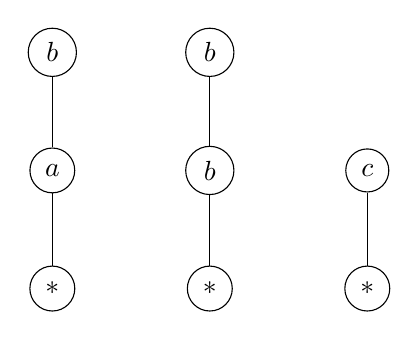
\begin{tikzpicture}
      \path
      (0,0) node[circle, draw](x){\(*\)}
      (0,1.5) node[circle, draw](y){\(a\)}
      (0,3) node[circle, draw](z){\(b\)};
      \draw (x) -- (y) -- (z);

      \path
      (2, 0) node[circle, draw](x){\(*\)}
      (2, 1.5) node[circle, draw](y){\(b\)}
      (2, 3) node[circle, draw](z){\(b\)};
      \draw (x) -- (y) -- (z);

      \path
      (4, 0) node[circle, draw](x){\(*\)}
      (4, 1.5) node[circle, draw](y){\(c\)};
      \draw (x) -- (y);
    \end{tikzpicture}
  \end{equation*}
  with \(a, b, c \in B\).
  We immediately deduce that \(\mu F\) can also be realized as the set of words over \(B\).
\end{example}

\begin{remark}
  Notice the importance of constant symbols.
  Indeed if a polynomial functor on \(\Set\) has no constant then it preserves the initial object 0 so by Remark \ref{rem:trivial_initial_algebra} the initial algebra is trivial.
 Equivalently one can observe that, without constant symbols, the set of closed terms is empty.
\end{remark}

\begin{example}
  Consider \(FX = X_\bot\) on \(\CPO_\bot\).
  Let \(\mathbb{N}^\top\) be the set of the natural numbers with an added topmost element \(\infty\) ordered naturally.
  Notice that \((\mathbb{N}^\top)_\bot\) is isomorphic (as an order) to \(\mathbb{N}^\top\) and consider the successor function \(s \colon (\mathbb{N}^\top)_\bot \to \mathbb{N}^\top\) with \(s(\infty) = \infty\).
  We claim this is the initial algebra for \(F\).

  Let \((A, \alpha)\) be another \(F\)-algebra and \(f \colon (\N^\top, s) \to (A, \alpha)\) a morphism.
  Because \(f\) is an arrow of \(\CPO_\bot\) it must be strict so \(f(0) = \bot\) and because it is a morphism we must have \(f(s(n)) = \alpha(f(n))\); this defines \(f\) inductively on \(\N\).
  Finally we recall that \(f\) must be continous (as an arrow of \(\CPO_\bot\)) so
  \begin{equation*}
    f(\infty) = f \left(\bigvee_{n < \omega} n\right) = \bigvee_{n < \omega}(f(n)).
  \end{equation*}
  This implies that there is really a unique morphism from \((\N^\top, s)\) to \((A, \alpha)\) so \((\N^\top, s)\) is initial.
\end{example}

We conclude this section with the a classic lemma of Lambeck's which gives necessary conditions for functors to have an initial algebra.

\begin{definition}
  A \textbf{fixed point} of an endofunctor \(F\) is an element \(A \in \mathscr{A}\) that is isomorphic to \(FA\).
\end{definition}

\begin{lemma}[Lambeck's Lemma]
  An initial algebra for \(F\) is always a fixed point.
\end{lemma}

\begin{proof}
  Let \((\mu F, \iota)\) be the initial algebra of \(F\).
  Notice that \((F(\mu F), F\iota)\) is also an algebra and so there is a unique morphism \(f \colon (\mu F, \iota) \to (F(\mu F), F\iota)\).
  We have that the following diagram commutes
  \begin{equation*}
    \begin{tikzcd}[sep = large]
      F(\mu F) \ar[r, "\iota"] \ar[d, "Ff"] & \mu F \ar[d, "f"]\\
      F(F(\mu F)) \ar[r, "F\iota"] \ar[d, "F\iota"]& F(\mu F) \ar[d, "\iota"]\\
      F(\mu F) \ar[r, "\iota"] & \mu F
    \end{tikzcd}
  \end{equation*}
  so \(\iota \circ f\) is an endomorphism of algebras on the initial algebra; hence it is \(\id_{\mu F}\).
  Now
  \begin{equation*}
    f \circ \iota = F\iota \circ Ff = F(\iota \circ f) = F(\id_{\mu F}) = \id_{F(\mu F)}
  \end{equation*}
  so \(\iota\) is an isomorphism.
  This shows that \(\mu F\) is a fixed point of \(F\).
\end{proof}

\begin{remark}
  We know from Cantor's Theorem that there is no surjection from a given set \(X\) into its power set \(\mathcal{P}X\) so the functor \(\mathcal{P}\) on \(\Set\) has no fixed point hence no initial algebra.
\end{remark}

Lambeck's lemma can be seen as a generalization of the following order-theoretic lemma.

\begin{definition}
  Let \((P, \sqsubseteq)\) be a poset and \(f \colon P \to P\) a monotone function.
  An element \(x \in P\) is a \textbf{pre-fixed point} of \(f\) if \(f(x) \sqsubseteq x\).
\end{definition}

\begin{lemma}
  \label{lemma:order_theory}
  Given a poset \((P, \sqsubseteq)\) and a monotone function \(f \colon P \to P\) let \(A = \{x \in P \colon f(x) \sqsubseteq x\}\) be the set of pre-fixed points of \(f\).
  If \(\overline{a}\) is the meet of \(A\) then \(\overline{a}\) is the least fixed point of \(f\).
\end{lemma}

\begin{proof}
  If \(x \in A\) then \(\overline{a} \sqsubseteq x\) and \(f(\overline{a}) \sqsubseteq f(x) \sqsubseteq x\) follows from monotony of \(f\) and definition of \(A\).
  This shows that \(f(\overline{a})\) is a lower bound for \(A\) so \(f(\overline{a}) \sqsubseteq \overline{a}\).
  Now by applying \(f\) again we obtain \(f(f(\overline{a})) \sqsubseteq f(\overline{a})\) which gives us \(f(\overline{a}) \in A\) and thus \(\overline{a} \sqsubseteq f(\overline{a})\).
  Moreover \(\overline{a}\) must be the least fixed point of \(f\) since all fixed points are pre-fixed points.
\end{proof}

This lemma then gives us the following well-known theorem for free.

\begin{theorem}[Knaster-Tarski Theorem]
  Let \((L, \sqsubseteq)\) be a complete lattice.
  Then every monotone function of \(L\) has a fixed point.
\end{theorem}

\begin{proof}
  Let \(f\) be a monotone function on \(L\) and \(A\) be the set of pre-fixed points of \(f\).
  It must have a meet \(\overline{a}\) because the lattice is complete so by the Lemma we have a fixed point.
\end{proof}

The generalization of order theoretic results such as Lemma \ref{lemma:order_theory} will be a recurrent theme.
Indeed we can see orders as categories in the usual way, order-preserving functions as functors and pre-fixed points as algebras for these functors.

\section{Recursion and Induction}

Recursion is a way of defining a function \(f\) on the natural numbers by specifying a value for \(f(0)\) and a way of deriving the value of \(f(n + 1)\) from the value of \(f(n)\).
Recursion, however, can also be used to define functions on (among other things) trees; in this case it is usually called \emph{structural} induction (we have an example of this in Remark \ref{rem:ev_function}).
Here we show how one can use the concept of an initial algebra to provide a general definition of recursion of which the cited examples as particular cases.

\begin{definition}
  Let \(F\) be an endofuctor and \(\mu F\) its initial algebra.
  A morphism \(f \colon \mu F \to A\) is \textbf{recursively specified} \marginnote{recursively specified} if there exists an algebra structure \(\alpha \colon FA \to A\) on \(A\) that makes \(f\) into an algebra homomorphism (actually the unique algebra homomorphism).
\end{definition}

\begin{example}
  Consider the functor \(FX = X \times X + 1\) on \(\Set\) and let \(T\) be its initial algebra that we know from Example \ref{ex:finite_binary_trees} is the algebra of finite binary trees with tree-tupling.
  Let \(h \colon T \to \mathbb{N}\) be the function that assigns \(0\) to the root-only tree and, given a tree \(t\) obtained by tree-tupling of \(t_1\) and \(t_2\), \(h(t) = 1 + \max\{h(t_1), h(t_2)\}\).
  We now show that \(h\) is recursively specified according to our definition.

  We need an algebra structure on \(\mathbb{N}\) i.e. an arrow \(\alpha \colon \N \times \N + 1 \to \N\).
  Since \(\alpha\) is an arrow out of a coproduct we have \(\alpha = [\alpha_1, \alpha_0]\) so we can let
  \begin{align*}
    \alpha_0 &= 0;\\
    \alpha_1(n, m) &= 1 + \max\{n, m\}.
  \end{align*}
  Indeed if \(\iota_1\) is tree-tupling and \(\iota_0\) is the root-only tree the following square trivially commutes thus \(h\) is recursively specified.
  \begin{equation*}
    \begin{tikzcd}[sep = large]
      T \times T + 1 \ar[r, "\outofcoprod{\iota_1}{\iota_0}"] \ar[d, "h \times h + \id_1"] & T \ar[d, "h"]\\
      \N \times \N + 1 \ar[r, "\outofcoprod{\alpha_1}{\alpha_0}"] & \N
    \end{tikzcd}
  \end{equation*}
\end{example}

The following theorem is a generalization of the classic recursion with parameters theorem.

\begin{theorem}[Primitive Recursion]
  \label{teo:primitive_recursion}
  Assume the base category \(\mathscr{A}\) to have finite products and let \(F\) be an endofunctor with an initial algebra \(\mu F\).
  Then for every \(\alpha \colon F(A \times \mu F) \to A\) there is a unique \(h \colon \mu F \to A\) such that the following square commutes.
  \begin{equation}
    \label{dia:recursion}
    \begin{tikzcd}[sep = large]
      F(\mu F) \ar[r, "\iota"] \ar[d, "F \intoprod{h}{\id_{\mu F}}"] & \mu F \ar[d, "h"] \\
      F(A \times \mu F) \ar[r, "\alpha"] & A
    \end{tikzcd}
  \end{equation}
\end{theorem}

\begin{proof}
  Let \(\pi_1, \pi_2\) be the projections of the product \(A \times \mu F\) and consider the arrow
  \begin{equation*}
    \overline{\alpha} \colon F(A \times \mu F) \xrightarrow{\intoprod{\id_{F(A \times \mu F)}}{F\pi_2}} F(A \times \mu F) \times F(\mu F) \xrightarrow{\alpha \times \iota} A \times \mu F.
  \end{equation*}
  This gives an algebra structure on \(A \times \mu F\) so let \(\overline{h} \colon \mu F \to A \times \mu F\) be the unique algebra homomorphism given by the initiality of \(\mu F\).
  \begin{equation}
    \label{dia:recursion2}
    \begin{tikzcd}[row sep = large, column sep = 6 em]
      F(\mu F) \ar[drr, phantom, "\scriptstyle (1)"] \ar[d, "F\overline{h}"] \ar[rr, "\iota"] & & \mu F \ar[d, "\overline{h}"] \\
      F(A \times \mu F) \ar[r, "\intoprod{\id_{F(A \times \mu F)}}{F\pi_2}"] \ar[drr, phantom, "\scriptstyle (3)", very near start] \ar[d, "F\pi_2"] & F(A \times \mu F) \times F(\mu F) \ar[r, "\alpha \times \iota"] \ar[dl, "\pi_2"] \ar[dr, phantom, "\scriptstyle (2)"] & A \times \mu F \ar[d, "\pi_2"] \\
      F(\mu F) \ar[rr, "\iota"] & & \mu F
    \end{tikzcd}
  \end{equation}
  The outer square in (\ref{dia:recursion2}) commutes because (1), (2) and (3) do.
  Indeed (1) commutes because \(\overline{h}\) is an algebra homomorphism, (2) by Notation \ref{not:product_arrows} and (3) because of Notation \ref{not:brackets}.
  By functoriality of \(F\) we then have that \(\pi_2 \circ \overline{h}\) is an endomorphism on the initial algebra thus \(\pi_2 \circ \overline{h} = \id_{\mu F}\).

  Now set \(h \coloneqq \pi_1 \circ \overline{h}\) so \(\overline{h} = \intoprod{h}{\id_{\mu F}}\).
  Extending (1) by \(\pi_1\) we obtain the following diagram that we know commutes.
  \begin{equation*}
    \begin{tikzcd}[row sep = large, column sep = 6 em]
      F(\mu F) \ar[rr, "\iota"] \ar[d, "F\overline{h} = F\intoprod{h}{\id_{\mu F}}"]& & \mu F \ar[d, "\overline{h}"] \ar[dr, "h"] & \\
      F(A \times \mu F) \ar[r, "\intoprod{\id_{F(A \times \mu F)}}{F\pi_2}"] & F(A \times \mu F) \ar[r, "\alpha \times \iota"] \times F(\mu F) & A \times \mu F \ar[r, "\pi_1"] & A
    \end{tikzcd}
  \end{equation*}
  But notice that
  \begin{equation*}
    \pi_1 \circ (\alpha \times \iota) \circ \intoprod{\id_{F(A \times \mu F)}}{F\pi_2} = \pi_1 \circ \intoprod{\alpha}{\iota \circ F\pi_2} = \alpha.
  \end{equation*}
  so we have (\ref{dia:recursion}).

  To prove uniqueness consider \(h \colon \mu F \to A\) homomorphism of algebras such that (\ref{dia:recursion}) commutes.
  We claim that \(\overline{h} = \intoprod{h}{\id_{\mu F}}\) so that \(h = \pi_1 \circ \overline{h}\); thus uniqueness.
  In order to do it we show that \(\intoprod{h}{\id_{\mu F}}\) is an algebra homomorphism and conclude it must be \(\overline{h}\) by initiality of \(\mu F\).
  Indeed we have
  \begin{align*}
    \pi_1 \circ (\alpha \times \iota) \circ \intoprod{\id_{F(A \times \mu F)}}{F\pi_2} \circ F\intoprod{h}{\id_{\mu F}}
    &= \alpha \circ \id_{F(A \times \mu F)} \circ F\intoprod{h}{\id_{\mu F}} \\
    &= h \circ \iota\\
    &= \pi_1 \circ \intoprod{h}{\id_{\mu F}} \circ \iota;\\
    &\\
    \pi_2 \circ (\alpha \times \iota) \circ \intoprod{\id_{F(A \times \mu F)}}{F\pi_2} \circ F\intoprod{h}{\id_{\mu F}}
    &= \iota \circ F\pi_2 \circ F\intoprod{h}{\id_{\mu F}}\\
    &= \iota \circ F(\pi_2 \circ \intoprod{h}{\id_{\mu F}})\\
    &= \iota \circ F\id_{\mu F}\\
    &= \iota \circ \id_{F(\mu F)}\\
    &= \iota\\
    &= \pi_2 \circ \intoprod{h}{\id_{\mu F}} \circ \iota;
  \end{align*}
  so we conclude by Proposition \ref{prop:arrows_into_limit}.
\end{proof}

Recall the classic recursion with parametes theorem.
We shall prove it using Theorem \ref{teo:primitive_recursion}; for a classical proof see \cite[Theorem 18.1]{andrettaelements}.

\begin{theorem}[Recursion with parameters]
  Let \(A\) be a set, \(a \in A\) and \(f \colon A \times \N \to A\) be a function.
  Then there is a function \(g \colon \N \to A\) such that
  \begin{equation*}
    \begin{cases}
      g(0) = a \\
      g(n + 1) = f(g(n), n)
    \end{cases}.
  \end{equation*}
\end{theorem}

\begin{proof}
  Consider the functor \(FX = X + 1\) on \(\Set\) and form the arrow
  \begin{equation*}
    \alpha \colon F(A \times \mu F) = A \times \N + 1 \xrightarrow{\outofcoprod{f}{a}} A.
  \end{equation*}
  Now by Theorem \ref{teo:primitive_recursion} there is a function \(g \colon \N \to A\) such that (\ref{dia:recursion}) commutes.
  This gives us the diagram
  \begin{equation}
    \begin{tikzcd}[sep = large]
      \N \times 1 \ar[r, "\outofcoprod{\iota_1}{\iota_0}"] \ar[d, "\intoprod{g}{\id_\N} + \id_1"] & \N \ar[d, "g"]\\
      A \times \N + 1 \ar[r, "\outofcoprod{f}{a}"] & A
    \end{tikzcd}
  \end{equation}
  that yields the conditions
  \begin{enumerate}
  \item[1.] \(g \circ \iota_0 = a \circ \id_1\);
  \item[2.] \(g \circ \iota_1 = f \circ \intoprod{g}{\id_\N}\).
  \end{enumerate}
  Now 1 gives us \(g(0) = a\) and 2 that
  \begin{equation*}
    g(n + 1) = (g \circ \iota_1)(n) = (f \circ \intoprod{g}{\id_\N})(n) = f(g(n), n) \quad \text{for all \(n < \omega\).}
  \end{equation*}
  So \(g\) has the required properties.
\end{proof}

The induction principle, that if a subset of \(\N\) contains \(0\) and is closed under the successor operation then it is \(\N\), can also be generalized to the more general setting of \(F\)-algebras.
Recall that a subobject in a category is represented by a monomorphism.
We call subalgebras subobjects in \(\alg F\).

\begin{theorem}[Induction Principle]
  Let \(F\) be an endofunctor and \(\mu F\) its initial algebra.
  Then every subalgebra of \(F\) is an isomorphism.
\end{theorem}

\begin{proof}
  Let \(m \colon (B, \beta) \to (\mu F, \iota)\) be a subalgebra.
  By initiality there is a unique homomorphism of \(F\)-algebras \(h \colon (\mu F, \iota) \to (B, \beta)\).
  Now \(m \circ h\) is an endomorphism of the initial object of \(\alg F\) so \(m \circ h = \id_{\mu F}\), but notice that we have \(m\) monic and split-epi thus an isomorphism.
\end{proof}

\chapter{Initial algebras from finitary iteration}
\newpage

\section{Adámek's Theorem}

We begin this section by recalling Kleene's Fixed Point Theorem and its proof with the goal of generalizing it to the categorical setting.

\begin{theorem}[Kleene's Fixed Point Theorem]
  \label{teo:kleene}
  Let \(A\) be a CPO with bottom \(\bot\); then every continous function \(F \colon A \to A\) has a least fixed point \(\mu F = \sup_{n < \omega}F^n(\bot)\)\footnote{We write \(F^n\) for \(\underbrace{F \ldots F}_{n \text{ times}}\) and \(F^0\) is the identity function. We use a similar notation for functors.}.
\end{theorem}

\begin{proof}
  Consider the \(\omega\)-chain \(\bot \leq F(\bot) \leq F^2(\bot) \leq \ldots\) and let \(\mu F\) be its join.
  By continuity \(F(\mu F) = \bigvee_{n < \omega}F(F^n(\bot))\) but we know that \(\bigvee_{n < \omega}F^n(\bot) = \bigvee_{n < \omega}F^{n+1}(\bot)\) so \(\mu F = F(\mu F)\), a fixed point.

  Now let \(F(x) \leq x\) be a pre-fixed point.
  As \(\bot \leq x\) we have \(F(\bot) \leq F(x) \leq x\) and by induction we obtain that \(F^n(\bot) \leq x\) for all \(n < \omega\) so \(x\).
  But this shows that \(x\) is an upper bound so \(\mu F \leq x\) by definition and, finally, \(\mu F\) must be the least fixed point because it is less than any pre-fixed point and fixed points are trivially pre-fixed points.
\end{proof}

Unsurprisingly we shall replace CPOs with bottom by categories with an initial obejct and endofunctions by endofunctors.
The \(\omega\)-chain used in the proof of Theorem \ref{teo:kleene} becomes a diagram and the continuity condition become a colimit-preservation one.

\begin{definition}
  The \textbf{initial-algebra \(\omega\)-chain}\marginnote{initial-algebra \(\omega\)-chain} of an endofunctor \(F\) is the diagram
  \begin{equation}
    \label{dia:initial_chain}
    \begin{tikzcd}[sep = large]
      0 \ar[r, "!"] & F0 \ar[r, "F!"] & F^20 \ar[r, "F^2!"] & F^30 \ar[r, "F^3!"] & \cdots
    \end{tikzcd}
  \end{equation}
  where we denote by \(!\) the unique arrow out of the initial object.
  This diagram can be realized as a functor from \(\omega\) regarded as a category.
\end{definition}

\begin{remark}
  \label{rem:induced_cocone}
  Let \((A, \alpha)\) be an \(F\)-algebra.
  Then it induces a canonical cocone \((\alpha_n \colon F^n0 \to A)_{n < \omega}\) on (\ref{dia:initial_chain}) by
  \begin{align*}
    \alpha_0 &=\ ! \\
    \alpha_{n+1} &= FF^n0 \xrightarrow{F\alpha_n} FA \xrightarrow{\alpha} A.
  \end{align*}
  To check that the \(\alpha_n\)'s are a cocone we prove \(\alpha_n = \alpha_{n+1} \circ F^n!\) by induction on \(n\).
  When \(n = 0\) the condition becomes \(! = \alpha_1 \circ !\) which is true because both sides are arrows out of the initial object.
  Now suppose the condition holds for \(n - 1\):
  \begin{align*}
    \alpha_{n+1} \circ F^n! &= \alpha \circ F\alpha_n \circ F^k! && \text{definition of \(\alpha_{n+1}\)}\\
    &= \alpha \circ F(\alpha_n \circ F^{n-1}!) && \text{functoriality of \(F\)}\\
    &= \alpha \circ F\alpha_{n-1} && \text{inductive hypothesis}\\
    &= \alpha_n && \text{definition of \(\alpha_n\)}.
  \end{align*}
\end{remark}

\begin{remark}
  If we apply \(F\) to the inital-algebra \(\omega\)-chain we obtain
  \begin{equation}
    \label{dia:initial_chain_F}
    \begin{tikzcd}[sep = large]
      F0 \ar[r, "F!"] & F^20 \ar[r, "F^2!"] & F^30 \ar[r, "F^3!"] & \cdots
    \end{tikzcd}.
  \end{equation}
  This \(\omega\)-chain has the same colimit as the original one.
  Indeed since the first element of (\ref{dia:initial_chain}) is the initial object there is an obvious one-to-one correspondence between cocones on (\ref{dia:initial_chain}) and cocones on the new chain above; and the same factorization morphisms work.
\end{remark}

We are ready to state and prove the main theorem of this chapter.

\begin{theorem}[Adámek]
  \label{teo:adamek}
  let \(\A\) be a category with an initial object \(0\) and colimits of \(\omega\)-chains and \(F\) an endofunctor that preserves \(\omega\)-colimits.
  Then \(F\) has an initial algebra \(\mu F = \colim_{n < \omega}F^n0\).
\end{theorem}

\begin{proof}
  Let \((\mu F, (c_n \colon F^n0 \to \mu F)_{n < \omega})\) be the colimit of the initial-algebra \(\omega\)-chain.
  Since \(F\) preserves \(\omega\)-colimits we have that \((F(\mu F), (Fc_n \colon F^{n+1} \to F(\mu F))_{n < \omega})\) is the colimit of (\ref{dia:initial_chain_F}) but \((c_{n+1} \colon F^{n+1}0 \to \mu F)_{n < \omega}\) is a cocone on (\ref{dia:initial_chain_F}) so there is a unique arrow \(\iota\) from \(F(\mu F)\) to \(\mu F\) such that
  \begin{equation}
    \label{eq:iota}
    \iota \circ Fc_n = c_{n + 1} \quad \text{for all \(n < \omega\).}
  \end{equation}
  This gives an \(F\)-algebra structure to \(\mu F\) that we now check is initial.

  Let \((A, \alpha)\) be a generic \(F\)-algebra.
  We have the induced cocone \((\alpha_n \colon F^n0 \to \mu F)_{n < \omega}\) as in Remark \ref{rem:induced_cocone} and this gives a unique arrow \(h \colon \mu F \to A\) such that \(h \circ c_n = \alpha_n\) for \(n < \omega\).
  We shall now prove that \(h\) is a morphism of \(F\)-algebras and that it is unique.

  To prove that \( h \circ \iota = \alpha \circ Fh\) we check that both arrows are factorization morphisms for the cocone \((\alpha_{n + 1} \colon F^{n+1}0 \to A)_{n < \omega}\).
  In practice we shall check that
  \begin{equation*}
    h \circ \iota \circ Fc_n = \alpha_{n + 1} = \alpha \circ Fh \circ Fc_n
  \end{equation*}
  for all \(n < \omega\).
  For the first equality notice that \(h \circ \iota \circ Fc_n = h \circ c_{n+1} = \alpha_{n+1}\).
  For the second equality consider the following diagram
  \begin{equation*}
    \begin{tikzcd}[sep = large]
      F^{n+1}0 \ar[r, "\alpha_{n+1}"] \ar[d, "Fc_n"'] \ar[dr, "F\alpha_n"] & A \\
      F(\mu F) \ar[r, "Fh"] & FA \ar[u, "\alpha"']
    \end{tikzcd}.
  \end{equation*}
  The upper-right triangle commutes by definition of \(\alpha_{n + 1}\) (see Remark \ref{rem:induced_cocone}).
  The lower-left triangle commute because \(h\) is the factorization arrow and by functoriality of \(F\).
  Then, as the whole square commutes, \(\alpha \circ Fh \circ Fc_n = \alpha_{n+1}\).
  This proves that \(h \colon \mu F \to A\) is a homomorphism of \(F\)-algebras.

  To prove uniqueness suppose there is an arrow \(k \colon \mu F \to A\) such that it is also an \(F\)-algebra homomorphism i.e. \(k \circ \iota = \alpha \circ Fk\).
  We will show that \(k \circ c_n = \alpha_n\) for all \(n < \omega\) and conclude by uniqueness of \(h\).
  Working by induction, if \(n = 0\) then \(k \circ c_0 = \alpha_0\) is trivial because both arrows are out of the initial object.
  Now suppose that \(k \circ c_n = \alpha_n\):
  \begin{align*}
    k \circ c_{n+1} &= k \circ \iota \circ Fc_n && \text{(\ref{eq:iota})}\\
    &= \alpha \circ Fk \circ Fc_n && \text{\(k\) homomorphism}\\
    &= \alpha \circ F(k \circ c_n) && \text{\(F\) functor}\\
    &= \alpha \circ F\alpha_n && \text{inductive hypothesis}\\
    &= \alpha_{n+1} && \text{definition of \(\alpha_{n+1}\)}.\\
  \end{align*}
  This concludes the proof.
\end{proof}

\begin{remark}
  Looking at the proof of Theorem \ref{teo:adamek} we notice that it isn't really necessary for \(\A\) to have colimits of \emph{all} \(\omega\)-chains or for \(F\) to preserve \emph{all} of them as we care for these properties only when applied to the initial-algebra \(\omega\)-chain.
  However in practice it may be more convenient to check the general properties rather than the particular case.
\end{remark}

\chapter{Initial algebras from transfinite iteration}
\newpage



\begin{tcolorbox}
  TODO: maybe intro on cardinals?
  TODO: find better name for this section.
\end{tcolorbox}

\section{Colimits of chains}

Through this chapter we regard ordinals \(j \in \Ord\) as linear orders and thus as categories.
A \(j\)-chain in some category \(\A\) is a functor \(C : j \to \A \)\marginnote{\(j\)-chain}; we denote the elements of the chain by \(C_i\), for \(i \in j\), and its arrows by \(c_{i,i'} : C_i \to C_{i'}\) for \(i \leq i' < j\).
We say that \(\A\) has colimits of chains if for all \(j \in \Ord\) every \(j\)-chain has a colimit; this includes the existence of an initial object (as the colimit of the empty chain) but does not include colimits of \(\Ord\)-chain.

\begin{lemma}
  \label{lemma:final_functors}
  Let \(j\) be an ordinal and \(C : j \to \A\) a \(j\)-chain into a category \(\A\) with colimits of chains. 
  Now let \(j' \subseteq j\) be cofinal i.e. such that for every \(i \in j\) there is some \(i' \in j'\) such that \(i \leq i'\) and denote by \(C'\) the restriction of \(C\) to \(j'\).
  Then \(C\) and \(C'\) have the same colimit.
\end{lemma}

\begin{proof}
  The first thing we notice is that there is a canonical bijection between cocones on \(C\) and cocones on \(C'\).
  Given a cocone \((A, \alpha_i : C_i \to A)_{i \in j}\) on \(C\) throwing away all the indexes not in \(j'\) yields \((A, \alpha_i : C_i \to A)_{i \in j'}\): a cocone on \(C'\).
  Conversely given \((A, \alpha_i : C_i \to A)_{i \in j'}\) we need to define \(\alpha_i : C_i \to A\) for all \(i \in j \setminus j'\); but there's only one way to do so.
  Indeed by cofinality let \(i' \in j'\) be such that \(i \leq i'\); then by the cocone condition we must set \(\alpha_i = \alpha_{i'} \circ c_{i,i'}\) so \((A, \alpha_{i}:C_i \to A)_{i \in j'}\) can be extended to the whole chain in only one way.

  Let \((L, \sigma_i : C_i \to L)_{i \in j}\) be the colimit of \(C\); then \((L, \sigma_i : C_i \to L)_{i \in j'}\) is the colimit of \(C'\).
  Let \((A, \alpha_i : C_i \to A)_{i \in j'}\) be a cocone on \(C'\) that we extend to a cocone on \(C\) as explained above.
  Now, since \(L\) is the colimit, let \(m \colon L \to A\) be the unique factorization arrow such that
  \begin{equation*}
    m \circ \sigma_i = \alpha_i \quad \text{for all \(i \in j\)}.
  \end{equation*}
  Particularly for all \(i \in j'\) so \(m\) is a factorization of \((A, \alpha_i : C_i \to A)_{i \in j'}\) through \((L, \sigma_i : C_i \to L)_{i \in j'}\).
  To prove it is unique let \(n \colon L \to A\) be such that \(n \circ \sigma_i = \alpha_i\) for all \(i \in j'\); we will show that \(n\) actually works for all \(i \in j\) and thus must be \(m\) by uniqueness.
  Let \(i \in j \setminus j'\) and \(i' \in j'\) such that \(i \leq i'\) by cofinality, then we have
  \begin{equation*}
    n \circ \sigma_i = n \circ \sigma_{i'} \circ c_{i, i'} = \alpha_{i'} \circ c_{i,i'} = \alpha_i.
  \end{equation*}
  For the converse let \((L, \sigma_i : C_i \to L)_{i \in j'}\) be the colimit of \(C'\).
  One can prove that the unique extension \((L, \sigma_i : C_i \to L)_{i \in j}\) is the colimit of \(C\) by a similar argument.
  Finally we have that \(C\) and \(C'\) have the same colimit (modulo restriction/extension) and that the factorization arrows are the same.
\end{proof}

Thanks to this lemma we can safely calculate colimits of chains, or apply Proposition \ref{prop:arrows_from_colimit}, on convenient cofinal subchains instead of on the full chain.
This allows us to ``skip'' limit ordinals because given \(j\) limit the subset \(\{i \in j : \text{\(i\) successor}\}\) is cofinal in \(j\).

\section{Transfinite iteration}

The main result of this section is again a generalization to the categorical setting of an order-theoretic result; this time from Zermeleo.
Let \(P\) be a chain-complete poset and \(f : P \to P\) an order-preserving map.
We can define an \(\Ord\)-indexed sequence by transfinite recursion as follows
\begin{align*}
  f^0(\bot) = \bot && \text{base case;}\\
  f^{j+1}(\bot) = f(f^j(\bot)) && \text{for all ordinals \(j\);} \\
  f^j(\bot) = \bigvee_{i < j}f^i(\bot) && \text{for limit ordinals \(j\).}
\end{align*}
This sequence is clearly a chain.

\begin{theorem}[Zermeleo]
  \label{teo:zermeleo}
  Let \(P\) be a chain-complete poset.
  Then every order-preserving \(f : P \to P\) has a lest fixed point \(\mu f\) and \(\mu f = f^j(\bot)\) for some \(j \in \Ord\).
\end{theorem}

\begin{proof}
  By Hartog's Lemma (insert here a reference) there is an ordinal \(i\) such that there is no injection \(i \rightarrowtail P\).
  Thus there are \(j < k < i\) such that \(f^j(\bot) = f^k(\bot)\) and we have \(f^j(\bot) \leq f^{j+1}(\bot) \leq f^k(\bot)\) because \((f^j(\bot))_{j\in\Ord}\) is a chain.
  So \(f(f^j(\bot)) = f^{j+1}(\bot) = f^j(\bot)\) hence \(f^j(\bot)\) is a fixed point.

  Now let \(x = f(x)\) be another fixed point.
  By transfinite induction we can prove \(x \geq f^i(\bot)\) for all \(i \in \Ord\) (similarly to what we did in Theorem \ref{teo:kleene}) thus when \(i = j\) we obtain \(x \geq f^j(\bot)\).
  This proves that \(f^j(\bot)\) is indeed the least fixed point of \(f\).
\end{proof}

In order to generalize this theorem and its proof we begin by defining a trasfinite version of the initial-algebra \(\omega\)-chain.
This will be a functor \(W : \Ord \to \A\) into a category \(\A\) with colimits of chains.
It is defined by transfinite recursion as follows.
\begin{align*}
  W_0 = 0 && \text{base case};\\
  W_{j+1} = FW_j && \text{for all ordinals \(j\)};\\
  W_j = \colim_{i < j}W_i && \text{for all limit ordinals \(j\)}.
\end{align*}
As for arrows \(w_{0,1}\) is the unique arrow \(0 \to W_1 = F0\) and \(w_{i + 1, j+1} = Fw_{i,j}\) for all \(i, j \in \Ord\).
When \(j\) is limit we have \(W_j = \colim_{i < j}W_i\) so we let \(\{w_{i,j}\}_{i < j}\) be the arrows forming the colimit cocone.
We are only missing \(w_{j, j+1}\) for \(j\) limit.
Such arrows are obtained using the universal property of \(W_j\).
First notice that we can leave out the initial object \(0\) and all the limit ordinals without changing the colimit i.e.
\begin{equation*}
  W_j = \colim_{i < j}W_i = \colim_{\text{\(i < j\) successor}}W_i
\end{equation*}
by Lemma \ref{lemma:final_functors}.
Now \((Fw_{i,j} : FW_i = W_{i+1} \to FW_{j} = W_{j+1})_{i < j}\) is a cocone on this reduced diagram.
Thus we obtain a unique factorization arrow \(W_j \to W_{j+1}\) that we declare to be our \(w_{j, j+1}\) so the definition of our transfinite chain can continue.
Notice also that, being the factorization arrow, \(w_{j, j_+1}\) is such that
\begin{equation}
  \label{eq:omega-to-omega-plus-one}
  w_{j, j+1} \circ w_{i+1, j} = Fw_{i, j} \quad \text{for all \(i < j\)}.
\end{equation}

We now generalize Remark \ref{rem:induced_cocone} to the transfinite case.

\begin{remark}
  \label{rem:induce-transfinite-cocone}
  Let \((A, \alpha)\) be an \(F\)-algebra; then it induces a cocone \((\alpha_i : W_i \to A)_{i \in \Ord}\) on \(W\) as follows.
  \begin{align*}
    \alpha_0 &=\ ! && \text{base case};\\
    \alpha_{i+1} &= \alpha \circ F\alpha_i && \text{for all ordinals i};
  \end{align*}
  for limit ordinals \(j\) we define \(\alpha_{j} : W_j \to A\) to be the unique factorization arrow such that \(\alpha_j \circ w_{i,j} = \alpha_i\) for all \(i < j\).
  In order for this construction to work we need to prove that, at stage \(j\), \((\alpha_i : W_i \to A)_{i < j}\) is a cocone i.e. that
  \begin{equation}
    \label{eq:cocone-condition}
    \alpha_i \circ w_{k, i} = \alpha_{k}
  \end{equation}
  for all \(k < i < j\).
  Assuming that all \(\alpha_i\)'s for \(i < j\) have been constructed we have that:
  \begin{itemize}
  \item[1.] for \(w_{0,1}\) condition (\ref{eq:cocone-condition}) is trivial;
  \item[2.] for \(w_{k, i}\) with \(i\) limit it is trivial by construction of \(\alpha_{i}\);
  \item[3.] for \(w_{i, i+1}\) with \(i\) limit we can prove (\ref{eq:cocone-condition}) holds by showing
    \[\alpha_{i+1} \circ w_{i, i+1} \circ w_{k, i} = \alpha_i \circ w_{k, i} =  \alpha_{k}\]
    for all \(k < i\) and conclude by uniqueness of \(\alpha_i\).
    It is enough to prove the relation for all \(k < i\) successors by Lemma \ref{lemma:final_functors} and indeed we have
    \begin{align*}
      \alpha_{i+1} \circ w_{i, i+1} \circ w_{k, i} &= \alpha \circ F\alpha_i \circ w_{i, i+1} \circ w_{k, i} && \text{definition of \(\alpha_{i+1}\)}\\
                                      &= \alpha \circ F\alpha_i \circ Fw_{k-1, i} && \text{(\ref{eq:omega-to-omega-plus-one})} \\
                                      &= \alpha \circ F(\alpha_i \circ w_{k-1, i}) && \text{functoriality of \(F\)}\\
                                      &= \alpha \circ F\alpha_{k-1} && \text{definition of \(\alpha_{i}\)}\\
                                      &= \alpha_k && \text{definition of \(\alpha_k\)}.
    \end{align*}
  \item[4.] for \(w_{i,i+1}\) with \(i\) non-limit we proceed inductively like in Remark \ref{rem:induced_cocone}; the base case is provided by item 1 if \(i\) is a natural number and by item 3 otherwise.
  \end{itemize}
  Finally we conclude that \((\alpha_i : W_i \to A)_{i \in \Ord}\) is well defined and a cocone on \(W\) since, as we just proved, for every \(j\) limit \((\alpha_i : W_i \to A)_{i < j}\) is a cocone.
\end{remark}

\begin{definition}
  We say that the inital-algebra chain \textbf{converges}
  \marginnote{converge of the initial-algebra chain}
  in \(\lambda\) steps if \(w_{\lambda, \lambda+1}\) is an isomorphism and that it converges in \textbf{exactly} \(\lambda\) steps when \(\lambda\) is the least such ordinal.
\end{definition}

We are now ready to state and prove the transfinite version of Adámek's Theorem.

\begin{theorem}
  \label{teo:adamek_transfinite}
  Let \(\A\) be a category with colimits of chains and \(F\) an endofunctor.
  If the initial-algebra chain of \(F\) converges in \(j\) steps then \(W_j\) is the initial algebra \(\mu F\) with structure given by
  \begin{equation*}
    (w_{j,j+1})^{-1} : W_{j+1} = FW_j \to W_j.
  \end{equation*}
\end{theorem}

\begin{proof}
  We only need to prove that \(W_j\) with the algebra structure given above is initial.
  To this end let \((A, \alpha)\) be an \(F\)-algebra and let \(h\) be the arrow \(\alpha_j : W_j \to A\) of the cocone induced by \((A, \alpha)\) in the sense of Remark \ref{rem:induce-transfinite-cocone}.
  We shall prove that \(h\) is the unique \(F\)-algebra homomorphism from \(W_j\) to \(A\).
  \begin{equation*}
    \begin{tikzcd}[sep=huge]
      W_{j+1} = FW_j \ar[r, "(w_{j,j+1})^{-1}"] \ar[d, "Fh = F\alpha_j"'] \ar[dr, "\alpha_{j+1}"] & W_j \ar[d, "h = \alpha_j"]\\
      FA \ar[r, "\alpha"] & A
    \end{tikzcd}
  \end{equation*}
  In the above diagram the lower left triangle commute by construction of \(\alpha_{j+1}\) and the upper right one because the \(\alpha_i\)'s form a cocone.
  Thus the outer square commutes i.e. \(h\) is an homomorphism.

  To prove that \(h\) is unique assume that \(k : W_j \to A\) is another homomorphism.
  We will show by transfinite induction that \(h \circ w_{i, j} = k \circ w_{i, j}\) for all \(i \leq j\) and then conclude by choosing \(i = j\).
  Notice that \(h \circ w_{i, j} = \alpha_j \circ w_{i, j} = \alpha_i\) so we are really interested in proving
  \begin{equation}
    \label{eq:a}
    \alpha_i = k \circ w_{i, j}
  \end{equation}
  for all \(i \leq j\).
  If \(i = 0\) then (\ref{eq:a}) is obvious because both sides of the equality are arrows out of the initial object.
  If we have \(\alpha_i = k \circ w_{i, j}\) then
  \begin{align*}
    \alpha_{i+1} &= \alpha \circ F\alpha_i && \text{definition of \(\alpha_i\)}\\
            &= \alpha \circ F(k \circ w_{i, j}) && \text{inductive hypothesis}\\
            &= \alpha \circ Fk \circ w_{i+1, j+1} && \text{fuctoriality of \(F\)}\\
            &= k \circ (w_{j,j+1})^{-1} \circ w_{i+1, j+1} && \text{\(k\) homomorphism}\\
            &= k \circ w_{i+1, j}.
  \end{align*}
  Finally if \(i\) is limit we know \(\alpha_i\) is the unique arrow such that \(\alpha_i \circ w_{s,i} = \alpha_s\) for all \(s < i\); so if we show that \(k \circ w_{i, j}\) does the same then we have (\ref{eq:a}).
  Indeed for \(s < i\) we have
  \begin{align*}
    k \circ w_{i, j} \circ w_{s, i} &= k \circ w_{s, j} && \\
                            &= h \circ w_{s, j} && \text{inductive hypothesis since \(s < i\)}\\
                            &= \alpha_j \circ w_{s, j} && \\
                            &= \alpha_s && \text{the \(\alpha_i\)'s are a cocone}.
  \end{align*}
  This concludes the proof.
\end{proof}

\printbibliography
\end{document}
